\documentclass[pdftex,10pt,a4paper,twocolumn]{article}
\title{\textbf{Developing a cellular automaton model for kidney morphogenesis}}
\author{Ben Lambert}
\usepackage[titletoc,toc]{appendix}
\usepackage[pdftex]{graphicx}
\usepackage{url,times}
\usepackage{graphicx}
\usepackage{epstopdf}
\usepackage{amsmath}
\usepackage[all]{xy}
\usepackage{pxfonts}
\usepackage{colortbl}
\usepackage{color}
\usepackage{subfigure}
\usepackage{gensymb}
\usepackage{ctable}
\usepackage[justification=centering]{caption}[2007/12/23]
\usepackage{longtable}
\usepackage{pst-func}
\usepackage{pst-math}
\renewcommand{\bibname}{Works Cited}
\usepackage{listings}
\usepackage{setspace}
\usepackage{algorithm}
\usepackage{bbm}

\newcommand{\HRule}{\rule{\linewidth}{0.5mm}}
\begin{document}

\twocolumn[
\maketitle
\doublespacing
\begin{@twocolumnfalse}
\begin{abstract}
\textbf{The development of the kidney involves the interaction between two distinct populations of cells: the metanephric mesenchyme and the epithelium of the Wolffian Duct. From E10.5-11 (in mouse organ cultures) a uretic bud (UB) of epithelium forms, which invades the space of the mesenchyme; later undergoing branching and extension which ultimately results in the components of a functioning kidney: the nephrons and collecting duct. In this paper a simple cellular automaton model is presented which recapitulates the initial emergence of the UB, along with its primary branching. In the model, metanephric mesenchyme cells release a chemo-stimulant GDNF (implicated from experiments), which diffuses throughout the simulation area, and is taken up by the epithelium cells, influencing their resultant behaviour.}
\end{abstract}
\end{@twocolumnfalse}
]

\section{Introduction}
The human kidney's primary function is to filter blood of waste products (mainly urea) from metabolism. The most important functional units of a kidney are nephrons, which are responsible for regulating the concentration of water and other solutes released in urine. In a nephron blood is filtered by the Glomerulus, and the filtrate then flows through a system of structures (the proximal tubule, loop of Henle and the distal tubule), where filtrates are selectively reabsorbed, then connects with a connecting duct which delivers the waste products to the ureter for excretion.

A fully developed human kidney is composed of 200,000 to 1.8 million nephrons, connected by a system of connecting ducts to the ureter, with the majority of the structure being formed during the embryonic stages of life ~\cite{hughson2003glomerular}. There are functional consequences for reduced nephron number, with evidence suggesting that this can cause hypertension and renal failure in adult life ~\cite{hoy2008nephron}. Furthermore, kidney and urinary tract congenital disorders are amongst the most common birth defects ~\cite{airik2007down}, with hypoplasia and dysplasia occurring in up to 1/200 births \cite{weber2006prevalence}. These are suggestive that biological and computational models which can help illuminate the cause, action and potential remedy of these types of disorder would be of value clinically.

Experimental work has focussed on animal models (mice, rats and fish) to study renal development. Broadly, there are two categories of experiment which have been undertaken: \textit{in vivo} studies of the effects of knock-out genes, and \textit{in vitro} studies of explanted kidney cells, grown in particular culture media. In particular, mouse studies have already demonstrated their relevance to the study of human kidneys. Dominant renal hypodysplastic kidneys, characteristic of a number of human renal disorders, display mutations in genes which were first discovered in the mouse ~\cite{LittleMMcMahon2012}.

During embryogenesis the early kidney is made up solely of undifferentiated cells, called the intermediate mesoderm (IM). These cells act as progenitors for all future nephron cells and collecting duct epithelium. At E9.5 in mouse studies the cells at the dorsal end of the organ form the epithelium of the Wolffian Duct extending in a rostro-caudal direction, with the rest of the cells maintaining their respective pluripotency ~\cite{CostantiniFKopan2010},\cite{saxen1987early}. Later on during development the remaining intermediate mesoderm becomes specialised along the rostro-caudal axis, with a relatively dense 'cloud' of mesenchyme forming at the caudal end ~\cite{CostantiniFKopan2010}, called the metanephric mesenchyme (MM).

At E10.5-11, due to factors released by the MM, there is an outgrowth of the epithelium, taking the form of a single discrete bud - the uretic bud (UB) - in normal organ development, which invades the MM ~\cite{CostantiniFKopan2010},\cite{LittleMMcMahon2012}. The UB then undergoes rounds of branching and extension, resulting in the branched structure of the collecting duct and its associated tubules. During this time, there are a nexus of reciprocal interactions which determine the specific nature of the branched structure. Factors produced by the epithelium also have a role to play in determining nephronic strcuture. In particular Wnt9b has been implicated in stimulating differentiation of mesenchymal cells proximal to the UB to form epithelium which acts as progenitors to nephrons. Normal development of the kidney's underlying structure stops at around parturition. Figure \ref{fig:real-branching} shows how branching of the initial uretic bud leads to the kidney structure.

\begin{figure*}[t] 
\centering
\scalebox{0.5} 
{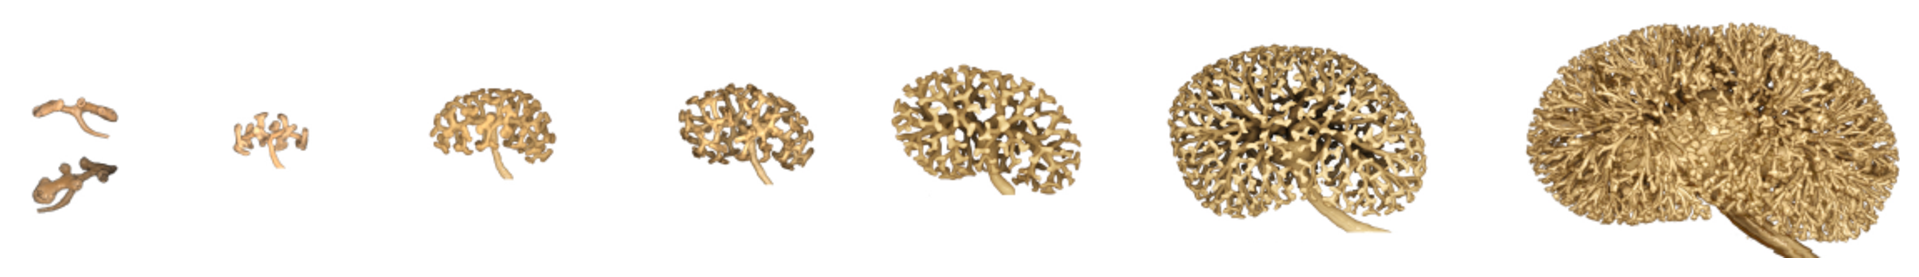
\includegraphics{real-branching.eps}}
\caption{This figure shows how the initial branching of the uretic bud (shown from two angles) on the left, can, via repeated branching and elongation, lead to the final kidney structure. This figure is taken from \cite{short2014global}.}\label{fig:real-branching}
\end{figure*} 

\section{GDNF stimulation of uretic bud growth}
There are a number of chemical signals produced by the metanephric mesenchyme which stimulate the growth of the uretic bud into the space occupied by the MM, and these have been reviewed comprehensively~\cite{costantini2006gdnf}, Dressler ~\cite{dressler2006cellular}. One of the most important of these factors is glial derived neurotrophic factor (GDNF), as GDNF$^{--}$ mutant mice typically do not produce uretic buds. Furthermore, this factor is the morphogen associated with driving the branching of the uretic bud.

GDNF is produced by the MM, and acts paracrinally on the epithelium; likely binding with two membrane surface Ret receptors (along with a co-receptor GFR$\alpha 1$) ~\cite{MenshykauDIber}. Ret$^{--}$ mice, like GDNF$^{--}$ mutants, (as well as GFR$\alpha 1$$^{--}$), fail to develop uretic buds ~\cite{CostantiniFKopan2010},\cite{majumdar2003wnt11},\cite{treanor1996characterization}, suggesting that a pathway involving these factors is involved in inducing the initial growth of the epithelium into the MM.

The chemo-attractive characteristics of GDNF ~\cite{tang2002ureteric},\cite{tang1998ret}, have led some to suggest that initial growth of uretic bud, as well as subsequent branching, is due, in part, to growth and movement of epithelium towards local GDNF sources \cite{sariola2003novel}. Furthermore, explanted epithelium cells have also been shown to grow additional uretic buds in the presence of beads soaked in GDNF \cite{pepicelli1997gdnf}. 

Ret has been shown to upregulate its own expression, as well as production of Wnt11 by the epithelium cells \cite{pepicelli1997gdnf}, which then regulates production of GDNF by the metanephric mesenchyme cells ~\cite{majumdar2003wnt11}. Thus production of GDNF exists in a feed-forward network, with reciprocal interactions between the epithelium and the mesenchyme cells. These interactions are displayed visually in figure \ref{fig:pathways}. GDNF expression is however tempered by a negative feedback loop involving \textit{Sprouty1} ~\cite{basson2005sprouty1}. FGF proteins have also been implicated in stimulating the emergence of the initial uretic bud, as well as branching, although it is likely that this process is less important than the GDNF mechanism, since FGFR2${^{--}}$ still undergo branching, albeit at a reduced level ~\cite{sims2009three}. However, in \textit{Sprouty1}${^{--}}$ mice, hyper-expression of FGF signalling proteins can generate phenotypically normal kidneys in GDNF$^{--}$ and Ret$^{--}$ mutants; which otherwise would have failed to develop kidneys at all. Since both Ret/GDNF and FGF10/FGFR have the same downstream targets ETV4/ETV5, it is likely that they may fulfil similar functions. This sort of redundancy could potentially have benefits evolutionarily.

\begin{figure*}[t] 
\centering
\scalebox{0.35} 
{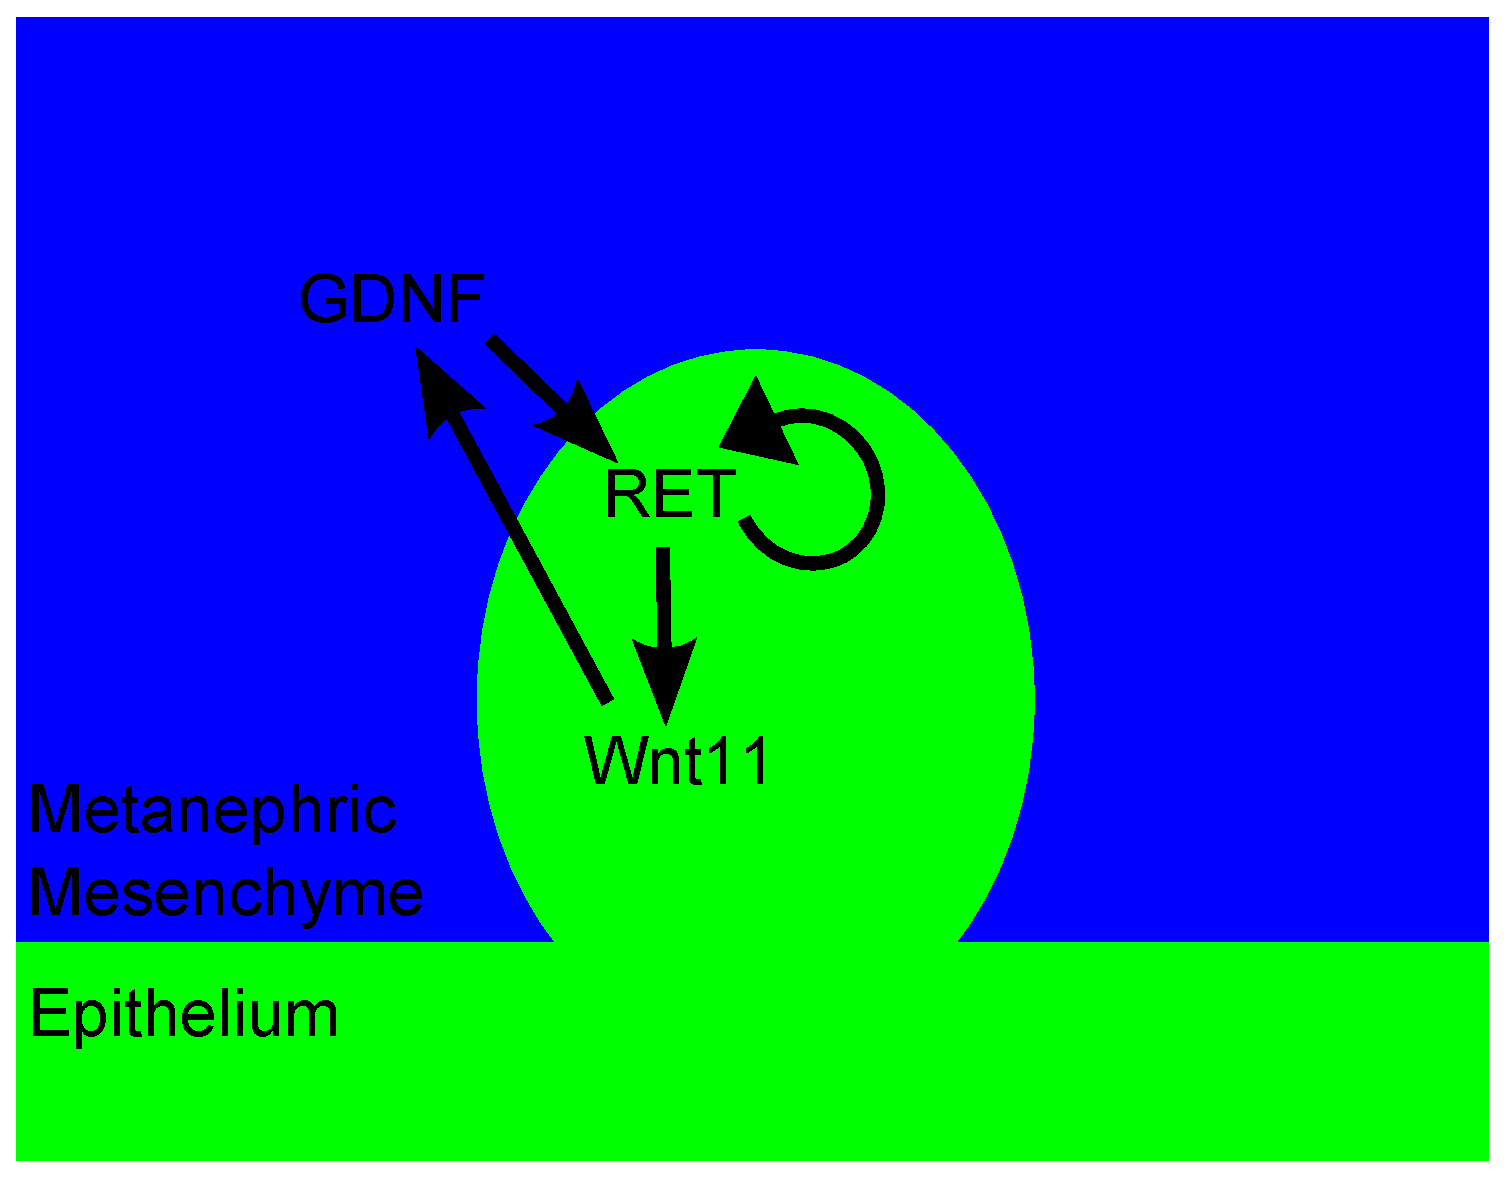
\includegraphics{pathways.eps}}
\caption{Shows the dominant reaction pathway for the regulation of GDNF in the developing kidney.}\label{fig:pathways}
\end{figure*} 

\section{Branching hypotheses}\label{sec:branchinghyp}
When the UB has invaded the MM, the UB undergoes approximately ten rounds of branching ~\cite{srinivas1999expression}. Subsequent to the initial branching, there is notable collecting duct lengthening, with one-two final rounds of branching before parturition ~\cite{cebrian2004morphometric}.

Branching of an emergent UB tip is witnessed in the absence of mesenchyme in explanted epithelium cells ~\cite{qiao1999branching}, however it is important to note that a culture medium containing GDNF, as well as medium derived from cells from the early metanephric mesenchyme are required for this to occur. Also, the branching morphology obtained with \textit{in vitro} explants is not the same as \textit{in vivo} patterning, suggesting that the mesenchyme-epithelium interaction at least plays a supporting role in kidney morphogenesis. Furthermore, experiments have been conducted whereby an explanted kidney epithelium is induced to branch like a lung, in the presence of lung mesenchyme \cite{lin2001induced}. However, the mesenchyme-independent branching result is suggestive that an important mechanism for branching is cell-contact-independent.

\begin{figure*}[t] 
\centering
\scalebox{0.2} 
{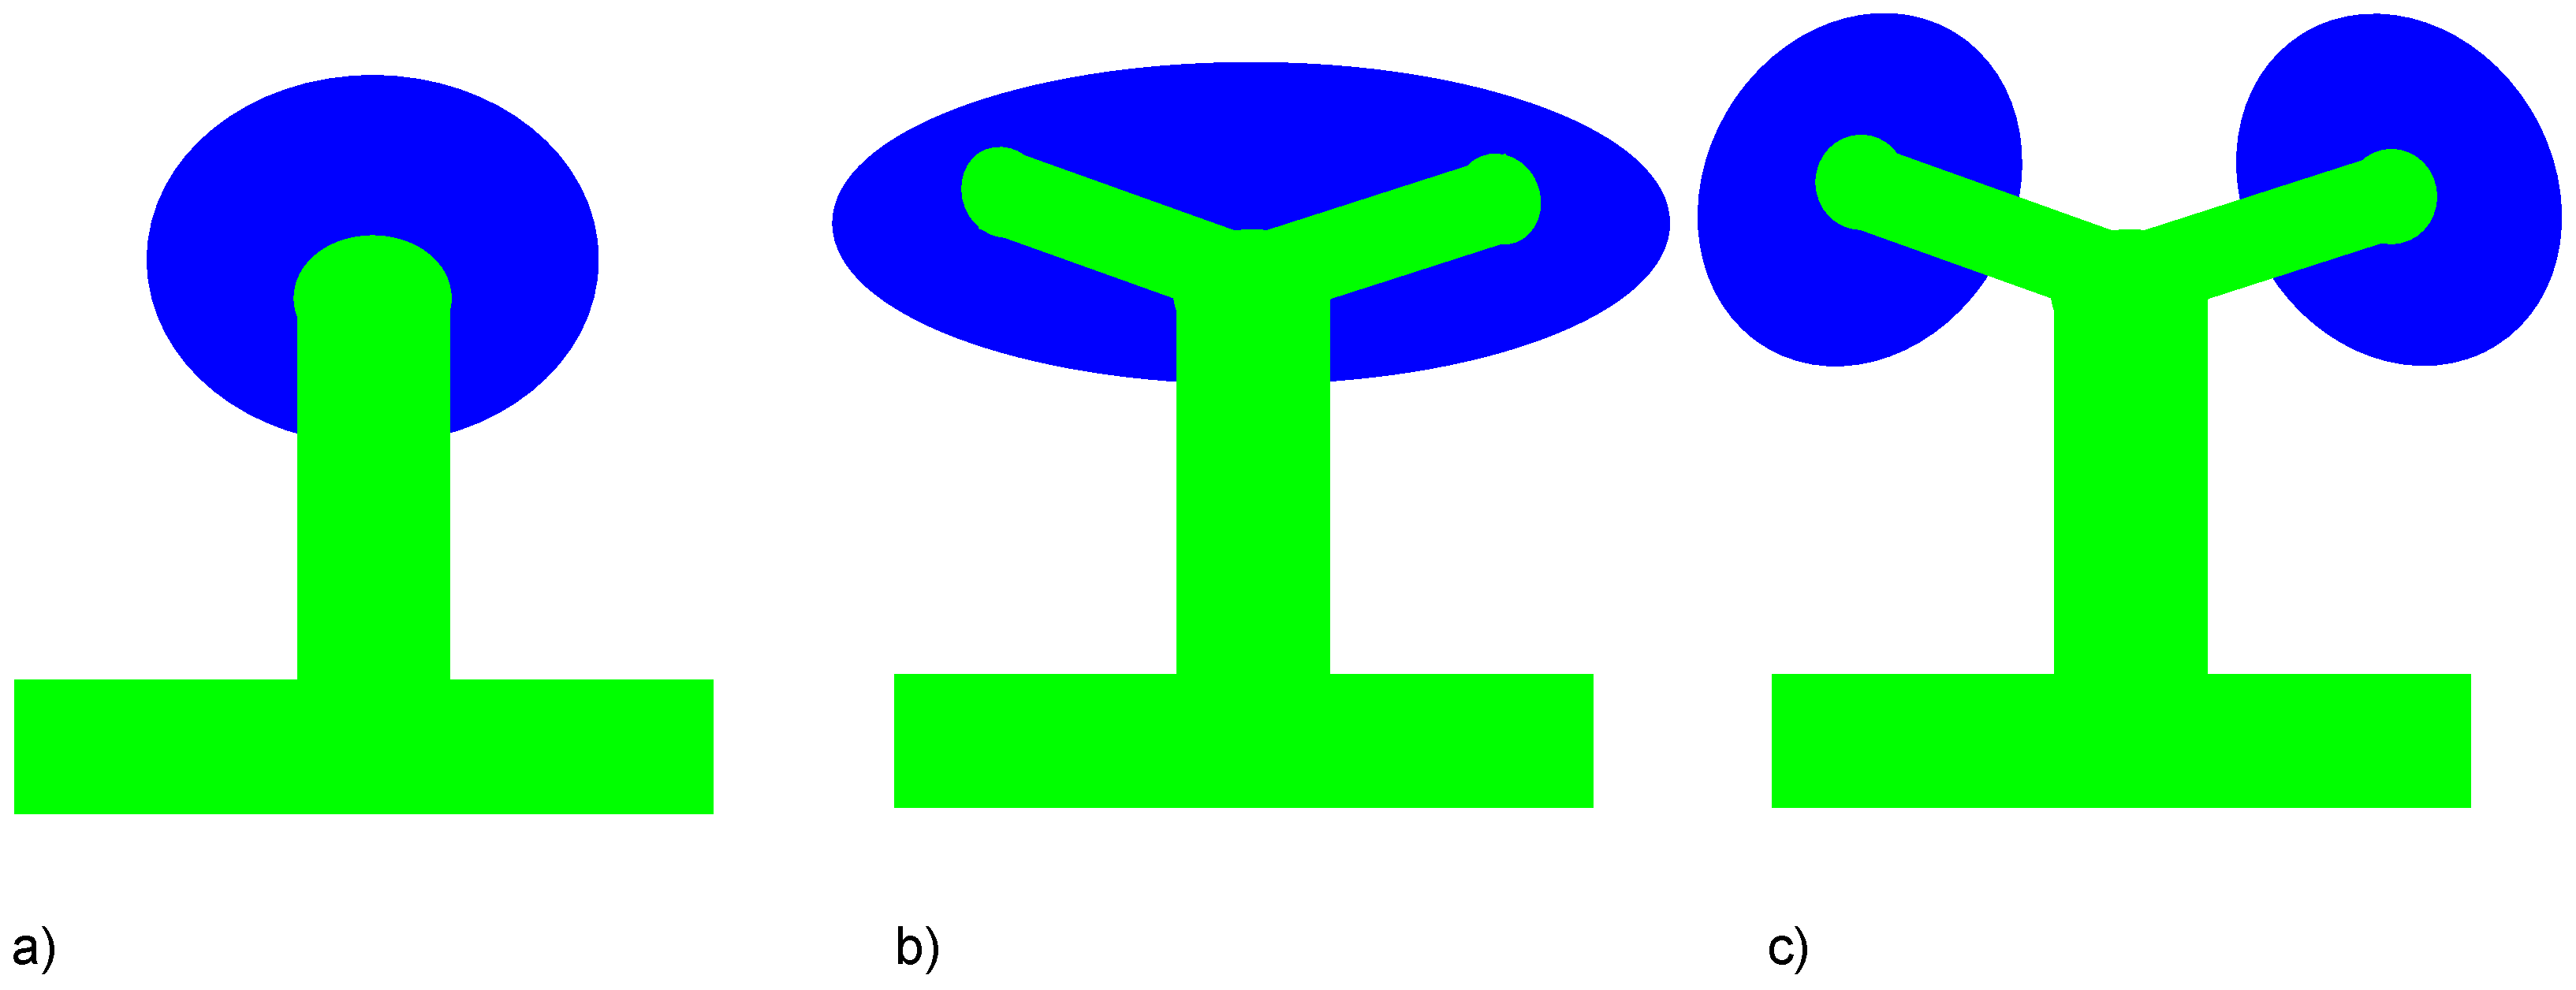
\includegraphics{UB_branch.eps}}
\caption{\textit{in vivo} branching, starting with an emergent UB in (a), initial branching occurring in (b), with discrete lobes of mesenchyme forming around epithelium tips in (c).}\label{fig:branch}
\end{figure*} 

The branches which are formed have (relatively) discrete masses of Six2$^+$ mesenchyme around their tips, with 'trunk' regions not having the same mesenchyme coverage \cite{short2014global}. It is not clear whether this is indicative of all mesenchyme cells, or simply those that are Six2$^+$. However, as a first approximation it may be important for a model of branching to generate these discrete lobes of mesenchyme around tip regions of epithelium, as shown in figure \ref{fig:branch}. 

The mechanisms which lead to the observed branching of epithelium in both \textit{in vivo} and \textit{in vitro} experiments is not well understood. The simplest hypothesis is that branching occurs as a result of local maxima and minima in GDNF, with epithelium cells 'attracted' towards the former \cite{sariola2003novel}. Continuum models which aim to recreate the positive feedback cycle shown in figure \ref{fig:pathways}, and allow growth of epithelium at a rate proportional to GDNF concentration, have been showing to recapitulate the branching seen \textit{in vivo} ~\cite{MenshykauDIber}. However, there are a number of issues with this approach. Firstly, if this system were allowed to continue to run, it would not necessarily reach a steady state where branching ceases, as is witnessed \textit{in vivo}. Secondly, although Ret is assumed to have a much lower diffusion rate than GDNF, since the former is a membrane protein, it is not clear whether free diffusion of Ret is a good assumption here. 

In reviewing potential mechanisms for branching Costantini and Kopan \cite{CostantiniFKopan2010} cast doubt on whether local proliferation of epithelium cells at the tips is an important mechanism since, "Mitotic events are diffusely distributed around the ampulla \cite{michael2004pattern}". They go on to suggest that three further mechanisms that could be the key to generating branching:

\begin{itemize}
\item Cell movements within the epithelium
\item Orientated cell division
\item Changes of cell shape
\end{itemize}

\begin{figure*}[t] 
\centering
\scalebox{0.2} 
{\includegraphics{UB_branch_ret.eps}}
\caption{\textit{in vivo} branching with Ret-high (in red) and Ret-low (in orange) shown.}\label{fig:branch_ret}
\end{figure*} 

The first of these three mechanisms is supported by the evidence that before a UB emerges, the epithelium cells sort themselves according to their level of Ret expression \cite{Chi2009}. Before the bud emerges, the Ret-high cells gather around the position of the future bud, then go on to form the tips of the UB. Ret-activity is necessary for epithelium cells to remain at the branching tips, as well as maintain branching capacity \cite{Chi2009}. Although Ret activity competition is evidently a part of \textit{in vivo} branching, it is still unclear as to how this mechanism would generate the branching that is seen. However, the discrete lobes of Six2-expressing mesenchyme which form around the tips (avoiding the trunks) could perhaps be explained by a different set of interactions between the Ret-high epithelium and the mesenchyme vs the Ret-low. A visualisation of this is shown in figure \ref{fig:branch_ret}.

Orientated cell division could be a potential candidate for a cause of branching, and is supported by the finding that tip cells proliferate in a different mechanism to those in the trunks ~\cite{packard2013luminal}. When the tip cells undergo mitosis, they produce a daughter cell in the lumen, which then reinserts somewhere into the epithelium not contiguous with the parent. Whereas trunk cells produce daughter cells which are adjacent to their parents \cite{packard2013luminal}.

Changes in cell shape have been suggested to be a potential cause of branching \cite{Meyer2004}. The authors propose a "purse-string" model, whereby a cell changes shape, and due to the mechanical effect of the microfilaments in epithelium cells, this can cause 'kinks' in the epithelium, resulting in branching.

As well as the qualitative aspects of branching that should be replicated, there are quantitative results which a successful model of kidney morphogenesis should be able to reproduce. Throughout developmental time, there are increases in both the number of epithelium tip and mesenchyme cells located in caps around the tips, although the rate of increase if the former is lower than the latter \cite{short2014global}. This results in a decrease in the ratio of the tip to cap cells throughout this time period. 


In summary, there are a number of mechanisms which are proposed for branching, although currently experiments are uncertain as to which (if any) of these is the primary driver of the branching morphology that is seen \textit{in vivo}.

\section{Differentiation of mesenchyme into nephron progenitors}
The nephrons of the kidney are formed when the mesenchyme cells surrounding tips of epithelium differentiate undergo a mesenchyme-to-epithelium-transition (MET) \cite{CostantiniFKopan2010}, \cite{LittleMMcMahon2012}. These epithelium cells then become renal vesicle cells, which attach themselves to the tips, and serve as progenitors for nephrons \cite{short2014global}. 

The mesenchyme cells which originally form around the tips are at a higher density than that of the surrounding MM, and is often termed the capping mesenchyme \cite{LittleMMcMahon2012}. The mesenchyme around tips is not homogeneous. Six2 expression in particular appears to vary dependent on the location of the mesenchyme cell, and has been demonstrated to be an important factor for maintaining mesenchyme cell pluripotency \cite{LittleMMcMahon2012}. In particular, Six2 knockout experiments in mice have demonstrated that there is premature transition of mesenchyme to renal vesicle progenitors; meaning nephrogenesis is severely impaired \cite{self2006six2}.

A number of signalling pathways have been suggested for inducing the transition of mesenchyme to epithelium cells. In mice Wnt9b signalling has been demonstrated to be the primary pathway for this induction \cite{LittleMMcMahon2012}, in particular isolated MM cells can be made to form renal vesicles in the presence of Wnt9b \cite{carroll2005wnt9b}. It is likely that Wnt9b is produced in the epithelium, and acts paracrinally on the surrounding mesenchyme cells. Since Six2 is required for mesenchyme cells to maintain their pluripotency, it is possible that a mechanism exists whereby Six2 acts to block the action of Wnt9b; preventing the cell differentiation into RVs \cite{LittleMMcMahon2012}. This would also explain why RVs tend to form in the 'armpit' region of branches, where the mesenchyme cells are surrounded by epithelium, and hence are exposed to the highest concentrations of Wnt9b.

\section{Cellular automaton model formulation}
A 2-dimensional simple cellular automaton model is presented where individual cell behaviour is governed by the identities of neighbouring cells and the local concentration of GDNF. Rules are chosen to govern cell-cell interactions as to replicate the behaviour seen in nature, as well as allowing all types of cell to occupy the same spatial area. These are both over-simplifications of the biological and physical mechanisms that govern the development of the kidney \textit{in vivo} and \textit{in vitro} for explants. However, it is hoped that the insight which this simple model can provide will be useful nonetheless for constructing more biologically and physically realistic models, where cellular behaviour is governed by physical laws rather than arbitrarily chosen rules. The model introduced here is an attempt to recapitulate branching and resultant mesenchyme distributions under the set of least restrictive assumptions, and resultant rules, as is possible.

\subsection{Basic model description}
The primary aim of this model is to recapitulate the development of the Uretic Bud \textit{in vivo} in 2D. However, it is also hoped that the model may be useful for the study of \textit{in vitro} explants. The details of the model are described in brief below:
\begin{itemize}
\item A 2 dimensional rectangular domain, assumed to be single occupancy, where each point in the array either represents the presence of:
\begin{itemize}
\item Epithelium cells - which consume GDNF
\item Metanephric mesenchymal cells (MM) - which produce GDNF
\item Extracellular matrix (ECM) - which allow for free diffusion of GDNF
\end{itemize}
\item Epithelium cells comprising either:
\begin{itemize}
\item A \textit{flat} membrane at the base of the simulation domain (aimed at recapitulating the \textit{in vivo} conditions from which the UB initially forms \textit{in utero}.)
\item A mass of epithelium cells with in general, curved boundaries, suspended towards the centre of the simulation domain (representative of the \textit{in vitro} explant experiment initial conditions.)
\end{itemize}
\item A diffuse collection of mesenchymal cells initially separate from the epithelium.
\end{itemize}


\subsection{GDNF field}
Cells in the MM produce GDNF, and it diffuses freely across the extracellular matrix (ECM) layer, and through the epithelium (being consumed by the latter). The reaction-diffusion type equation here will be assumed to be in equilibrium, since the diffusive timescale of GDNF is much less than that of the timescale of cell division. As such, the following is the form of the equation being solved:

\begin{equation}\label{eq:diffnorm}
D_G \nabla^2 = \Phi_G
\end{equation}

Where in (\ref{eq:diffnorm}) $D_G$ refers to the diffusion coefficient for GDNF, and $\Phi_G$ is the local rate of GDNF production or consumption (dependent on whether the cell in question is epithelium or mesenchyme). Specifically the rate of GDNF consumption is assumed to have the following form:

\begin{equation} \label{eq:production}
\Phi_G =\begin{cases}
K_G G, & \text{for epithelium}.\\
-\rho_G, & \text{for mesenchyme}.\\
0, & \text{for the extracellular matrix}.
\end{cases}
\end{equation}

It is assumed that the rate of GDNF consumption is linearly-dependent on the concentration of substrate. This assumption is likely violated when the GDNF concentration is high, and the cell Ret-receptors are saturated. In biologically realistic systems, it may be better to assume a Hill-type reaction rate. (Although it is unclear as to what range of concentrations of GDNF are likely to saturate the Ret receptors, and whether these are likely to be encountered either \textit{in vivo} or in experiments conducted thus far \textit{in vitro}.) It is assumed that the GDNF production rate by MM cells is a constant. This is not what occurs \textit{in vivo}, where the positive feedback mechanism shown in figure \ref{fig:pathways}, results in more GDNF being produced in the presence of Wn11; itself indirectly upregulated by GDNF. However, \textit{in vivo} this positive feedback mechanism is likely tempered by the \textit{Sprouty1} pathway (which itself is not fully-understood), and in \textit{in vitro} experiments without mesenchyme, branching occurs regardless. As such, the model presented here leaves out this feedback mechanism as a simplification.

The equation in (\ref{eq:diffnorm}) is non-dimensionalised using the following transformations:
\begin{equation}\label{eq:difftrans1}
\eta = \frac{x}{\Delta}
\end{equation}

\begin{equation}\label{eq:difftrans2}
g = \frac{G}{G_x}
\end{equation}

Where in (\ref{eq:difftrans1}) $\Delta$ refers to the typical cell dimensions (approximated as 5 $\mu m$),and $G_x$ is the concentration of GDNF typically found \textit{in vivo} (a value is currently not assigned here, since it is not strictly necessary for the non-dimensionalised simulation). These transformations result in the following non-dimensional form of the steady-state reaction-diffusion equation:

\begin{equation}\label{eq:diff-dimensionless}
\nabla_\eta^2 g = \frac{\phi_g}{d_g}
\end{equation}

Where in (\ref{eq:diff-dimensionless}), $d_g = \frac{D_G}{K_G \Delta^2}$, $\phi_g = \frac{\Phi_G}{K_G G_x}$, and $\nabla_\eta^2$ is the laplacian in the non-dimensional $\eta$ spatial coordinates.

The boundary conditions which are assumed are: no-flux at the base of the Wolffian Duct and top of the simulation domain, and periodic boundary conditions at either width. The simulation domain is chosen to be sufficiently large however, such that edge effects are not a primary driver of resultant behaviour. A finite difference approximation is used, with the no-flux boundary conditions at the top and bottom of the domain represented by the following relations for the non-dimensional GDNF field:

\begin{align*}
g_{0,j}& = g_{1,j}\\
g_{M,j}& = g_{M+1,j}\\
\end{align*}

where this holds $\forall j = 1,...,N$. $M$ here is the depth of the simulation domain in terms of cell dimensions. Similarly, for the periodic boundary conditions:

\begin{align*}
g_{i,0}& = g_{i,N}\\
g_{i,N+1}& = g_{i,1}\\
\end{align*}

where this holds $\forall i = 1,...,M$. $N$ here is the width of the simulation domain in terms of cell dimensions.

The finite-difference approximation for solving the steady-state reaction-diffusion equation is hence of the form:

\begin{equation}\label{eq:finitediff}
g_{i+1,j} + g_{i-1,j} + g_{i,j+1} + g_{i,j-1} - (4 + \epsilon_{i,j})g_{i,j} = -\psi_{i,j}
\end{equation}

Where in (\ref{eq:finitediff}):
\begin{equation}
\epsilon_{i,j} =\begin{cases}
\frac{1}{d_g}, & \text{for epithelium}.\\
0, & \text{for mesenchyme}.\\
0, & \text{for the extracellular matrix}.
\end{cases}
\end{equation}

Also, in (\ref{eq:finitediff}):
\begin{equation} \label{eq:psi}
\psi_{i,j} =\begin{cases}
0, & \text{for epithelium}.\\
\frac{\gamma}{d_g}, & \text{for mesenchyme}.\\
0, & \text{for the extracellular matrix}.
\end{cases}
\end{equation}

Where in (\ref{eq:psi}), $\gamma = \frac{\rho_G}{K_G G_x}$ captures the relative rate of GDNF production by the mesenchyme compared to the rate of GDNF consumption by epithelium under normal cellular conditions. It is assumed that $\gamma = 1$ in the simulations, in the absence of information regarding the relative weight of these two mechanisms. The diffusion rate constant, $D_G$, is assumed to be 10 $\mu m^2 s^{-1}$ \cite{MenshykauDIber}. If we assume that the diffusive time scale is similar to that of the consumption rate of GDNF we find that:

\begin{equation}\label{eq:diffusiontime}
k_G \sim \frac{D_G}{\Delta_{domain}^2} 
\end{equation}

Where in (\ref{eq:diffusiontime}), $\Delta_{domain}$ refers to the simulation domain spacial dimensions. 

In the simulation, it is assumed that the GDNF field does not vary significantly within a particular time step. As such (in order to reduce computational load), the GDNF field is only updated at the end of each time step, not after each cell movement or proliferation.

\subsection{Epithelium behaviour}
In this section the allowed behaviours of the epithelium cells in the cellular automaton model are described. In the simulation, each epithelium cell is visited in a random order, together with mesenchyme cells, and updated at each discrete time step according to the following pseudo-algorithm:

\begin{itemize}
\item \textit{Available cells} - Are neighbouring cells available for movement or proliferation? If yes, proceed to step 2. If no, move on to next cell. 
\item \textit{Move or proliferate} - Draw a random number $X\sim unif(0,1)$. If $P_{move}>X$ then proceed to \textit{move}. If not, proceed to \textit{proliferate}.
\item \textit{Move} 
\begin{enumerate}
\item \textit{Calculate the probability that a move takes place, $P_m$} - Based on a function of the local GDNF concentration. 
\item \textit{Does a move take place?} - Draw a random number $X\sim unif(0,1)$. If $P_{m}>X$ then proceed to next step. Otherwise, consider next epithelium cell.
\item \textit{Calculate probability of moving to each of the available cells} 
\item \textit{Choose amongst the available cells in accordance to their probability and move the cell in question}.
\end{enumerate} 
\item \textit{Proliferate}
\begin{itemize}
\item The framework is exactly analogous to that of \textit{Move} detailed above. In proliferation, the mechanism is slightly different due to the fact that a daughter cell is created in the target cell, rather than a cell simply moved there.
\end{itemize}
\item Consider next cell, returning to first step.
\end{itemize}

\subsubsection{Available neighbouring cells}\label{sec:available}
An epithelium cell's neighbours were chosen to be those grid points adjacent to the cell which were up, down, left or right of it. The simulations were also carried out using all points of a compass as representing as cell's neighbours, but there was not noticeable difference between the results, so the former rule was chosen. 

\begin{figure*}[t] 
\centering
\scalebox{0.5} 
{\includegraphics{connected.eps}}
\caption{An explanation of 'connectivity' for epithelium cells. All cells here are epithelium, the one highlighted in red is the cell which has been moved. The first two moves would be allowed, whereas the last is not.}\label{fig:connected}
\end{figure*} 


In reality the epithelium mass is a contiguous mono-layer of cells in the Wolffian duct (although the epithelium layer actually becomes pseudostratified before the UB forms \cite{Chi2009}). As such, there are likely cell-cell adhesion 'forces' that ensure that the cells do not frequently detach from the layer, and become isolated. There are also likely mechanical forces which restore the layer to a linear layer in the absence of other forces which may force it to buckle and curve. To ensure contiguity of the epithelium mass, an epithelium cell is only allowed to move into, or create a daughter cell in (proliferate), a neighbouring cell if it is 'connected' to other epithelium cells. I define a cell to be 'connected' if one or more of its neighbours is an epithelium cell. For a visual explanation of connectivity, see figure \ref{fig:connected}. Although this layer is \textit{in rerum natura} mono-layered, I choose to use a multi-layered epithelium. This is to allow for the fact that the simulation domain is two dimensional whereas in practice it is three dimensional. Making the layer multi-layered allows cells which are outside of the simulation plane to pass into the layer bordering on the ECM/mesenchyme.

A neighbouring cell is deemed available if it is vacant, or is occupied by a mesenchyme. For the latter case, the epithelium is only allowed to move into its spot if there is an allowed vacant position available into which the mesenchyme can be moved. The details of what is classed as an 'allowed' position for the mesenchyme being passively moved by encroaching epithelium are detailed in \ref{sec:mesenchyme}.

\subsubsection{Probability that a move or proliferation takes place}
Beads soaked in GDNF can induce the growth of additional buds \cite{pepicelli1997gdnf}, and GDNF$^{--}$ mutant mice fail to develop uretic buds ~\cite{CostantiniFKopan2010},\cite{majumdar2003wnt11},\cite{treanor1996characterization}. Hence it is likely that GDNF either directly or indirectly acts as a growth stimulant. In order to model GDNF's effect on growth, the probability that an epithelium cell undergoes a proliferation or movement is chosen to be modelled using a probit model:
\begin{equation}\label{eq:probit}
P(action) = \Phi(c_1 + c_2 g)
\end{equation}
Where in (\ref{eq:probit}), $\Phi$ is the standard normal CDF, and $action$ can either be a move or a proliferation event. This choice has the nice property that its output is constrained to be between 0 and 1. Furthermore, by choosing the parameter values $c_1$ and $c_2$, the function can essentially act as a binary switch, whereby above a certain GDNF concentration, cells always proliferate, and below it, they do not. This choice of parameters is essential to ensure that a discrete uretic bud emerges, rather than a general 'swelling'.

\subsubsection{Choosing between available target cells}
It is not clear whether GDNF-stimulated growth and movement of epithelium cells is sufficient to reproduce the branching morphologies that are seen, or whether it is necessary to orientate the processes towards local sources of GDNF. This directed movement of cells could be thought of as chemotaxis (in the case of movement), and a type of orientated cell division (in the case of proliferation).

In the model, this type of directed movement is handled by use of a multinomial probability distribution over choice of target cells (either for the epithelium to move into, or for a daughter cell to be created in the case of proliferation):

\begin{equation} \label{eq:multilogit}
P(target_n) = \frac{exp(c_3 + c_4(g^{target_n} - g^{current}))}{\sum\limits_{all targets} exp(c_3 + c_4(g^{target} - g^{current}))}
\end{equation}
Where in (\ref{eq:multilogit}), the benefit of this particular form is that the probabilities across all potential target cells for the epithelium naturally sum to 1. The parameter $c_4$ controls the extent to which the movement is directed towards local sources of GDNF, with a large parameter value strongly favouring those target cells which have higher levels of GDNF.

Although this type of discrimination between target cells is implemented in the simulation, in practice it does not appear to make qualitative changes in the distributions of epithelium and mesenchyme obtained. Hence, in order to simplify the simulations, further work was conducted without any directed choice of target cells for the epithelium.

\subsubsection{Ret-competition and transformation}
A potential cause of branching behaviour highlighted by Costantini and Koplan \cite{CostantiniFKopan2010}, is cell movements within the epithelium. In section \ref{sec:branchinghyp}, it was indicated that one potential source of epithelium heterogeneity, resulting in different movement behaviours across cells, could be through the expression of Ret. Furthermore, it was indicated that Ret-activity, specifically competition, occurs \textit{in vivo}, which results in Ret-high cells forming the initial bud, and then remaining in the tip cells \cite{Chi2009}. As such, two types of epithelium cell were created: Ret-high, and Ret-low. The former being more likely to divide and move in the presence of GDNF (this behaviour was elicited by allowing each cell type to have different parameter values in (\ref{eq:probit})).

As well as allowing Ret-high cells to move, and proliferate into neighbouring available cells at rates which are higher than the Ret-low, in order to reproduce the initial congregation of Ret-high cells which forms the uretic bud it was necessary to create a new type of behaviour. 'Competition' between a neighbouring Ret-high and Ret-low cell, if successful, results in the swapping of their respective cell positions. Successful competition can only occur probabilistically if the adjacent Ret-low cell is at a higher local GDNF concentration than the Ret-high one. The probability of swapping cell positions on the lattice is again determined by a probit function of the same form as (\ref{eq:probit}), with the move more likely to occur if the target cell has a higher concentration of GDNF. In the case of where two or more Ret-low cells are adjacent to a Ret-high cell, the cell with the highest GDNF concentration is chosen to be its 'partner' in competition.

The fates of epithelium cells are non in reality determined at their genesis \cite{CostantiniFKopan2010}. Lateral branching \cite{watanabe2004real}, and MM-induced branching \cite{sweeney2008developmental}, can both occur where new tips are formed from the trunk region of epithelium cells. As such, cells should be able to transform from one level of Ret expression into another. In order to allow transitions in both directions, the probabilities of a transition occurring (each time a cell is updated in the simulation), are of the probit form:

\begin{equation}\label{eq:transition}
P(transition) = \Phi (c_1 + c_2 g)
\end{equation}

Where in (\ref{eq:transition}) for the two cell types: $c_2>0$ for Ret-low to Ret-high transitions; and $c_2<0$ for Ret-high to Ret-low transitions. The differential transition probabilities for both cell types at a non-zero GDNF concentration allows for the creation of Ret-high cells in newly formed tips, and the transition of cells in stalk regions to Ret-low.

Finally, in order to form discrete lobes of mesenchyme around the tips (where the Ret-high cells are located), it is necessary for the mesenchyme to be attracted differentially to Ret-high and Ret-low cells respectively. The details of the rules governing this behaviour of mesenchyme are covered in section \ref{sec:mesenchyme}.

\subsubsection{Initial epithelium layer choice}
An adequate model of branching of uretic buds should be able to demonstrate branching \textit{in vitro} experiments, as well as \textit{in vivo} conditions. The typical type of \textit{in vitro} experiment set-up is an explanted uretic bud suspended in a culture of GDNF and a medium with 'essence' of cells derived from the early metanephric mesenchyme \cite{qiao1999branching}. This type of experiment demonstrates that branching can occur even in the absence of mesenchyme.

In order to recreate the initial transplanted UB in \textit{in vitro} experiments, an initial 'randomised' mass of epithelium cells (smoothed so that its edges were not overly jagged), was created in the middle of the simulation domain. This contrasted with the \textit{in vivo} case where an initial rectangular layer of epithelium cells with a depth of 20 cells was created.

\subsection{Mesenchyme behaviour}\label{sec:mesenchyme}
\subsubsection{Passive movement by encroaching epithelium}\label{sec:mespassive}
In section \ref{sec:available}, it was indicated that an epithelium cell can move into the position occupied by a mesenchyme if there is an allowed position into which it can itself be moved. However, it was not indicated what the use of 'allowed' meant in this case. Initial simulations where mesenchyme could only be moved into neighbouring cells caused a number of unrealistic features to result. Firstly, the incident epithelium layer was unable to move or penetrate a layer of mesenchyme cells which was greater than two cells in depth; instead the epithelium cells 'flowed around' the mesenchyme layer. Secondly, by virtue of the described 'flowing' behaviour of the epithelium, this meant it was often the case that islands of mesenchyme would be surrounded by a sea of epithelium; again not a biologically realistic situation. A solution to both of these issues was to allow mesenchyme cells to be moved non-locally into vacant cells in a field of cells determined by the direction from which the mesenchyme are being pushed. The number of positions considered depends on the number of moves forward allowed in the principal axis direction, and sideways along the secondary axis. These two axes are defined in figure \ref{fig:axes}. 

Although, this behaviour is less realistic than local movements, (as cells do not simply jump position), it can be thought of as representing the process whereby displacement of mesenchyme occurs via contact with epithelium, causing a movement of the entire mass. Since the mesenchyme cells are not heterogeneous in terms of their properties, in terms of the model, the movement of an individual cell non-locally to a position which is vacant is equivalent to a shuffling of the mesenchyme mass which results in an 'outer' mesenchyme occupying the same vacant position (assuming all other positions are the same between the two.) Furthermore, since the process causing the movement of the mass of mesenchyme is likely mechanical, its time scale can be thought of as faster than the general movement of cells; lending some justification for non-local jumping as representing movements which occur at a faster rate than cell movement or proliferation.

\begin{figure*}[t] 
\centering
\scalebox{0.35} 
{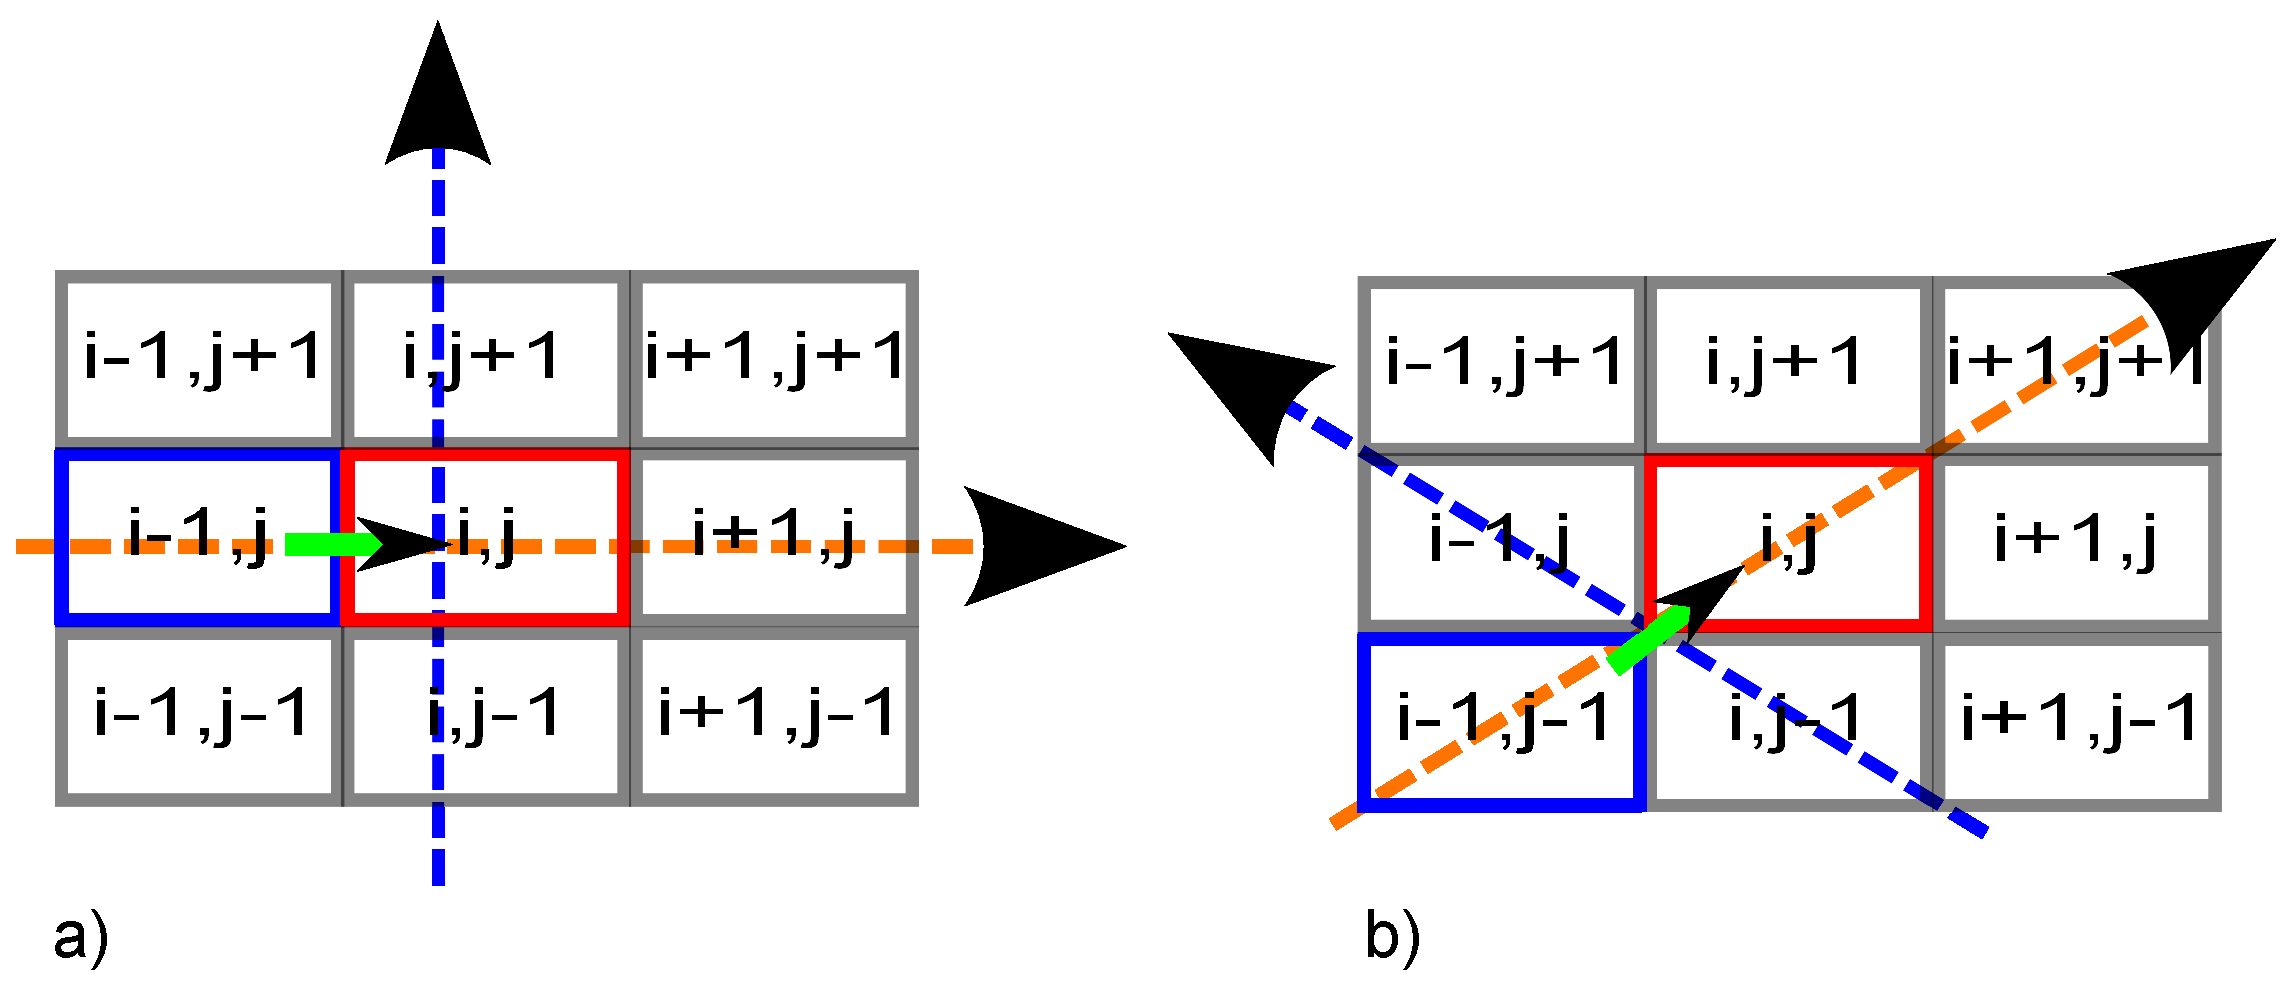
\includegraphics{axes.eps}}
\caption{The principal axis (in orange) and secondary axis (in blue) for two example movements. In a) the movement vector is horizontal, whereas in b) it is diagonal. The axes are not visually perpendicular in b) due to the fact that the cells are represented as rectangles rather than squares.}\label{fig:axes}
\end{figure*} 

\subsubsection{Active movement and proliferation}
In order to allow for condensation of mesenchyme around tips to occur, mechanisms for movement and proliferation of mesenchyme cells is allowed to occur probabilistically. The probability of a move or proliferation occurring is assumed to be dependent on their distance from the nearest epithelium cell. The pseudo-algorithm which is implemented is of the form:

\begin{enumerate}
\item Calculate the probability that a move/proliferation occurs. This is negatively related to the distance of each of the target cells to the nearest epithelium.\label{point:mesactive}
\item Draw a pseudo-random $X\sim unif(0,1)$. If $X<P(action)$ then proceed to the next step. If not, then proceed to the next epithelium/mesenchyme in the simulation time step.
\item Find all the possible targets for the mesenchyme cell from the 8-nearest-neighbours which are currently vacant. 
\item Select one from the set of targets probabilistically (using a multinomial logistic distribution), with targets further away from the epithelium penalised heavily in terms of their selection probability.\label{point:mesactive1}
\end{enumerate}

Two mechanisms allow for the epithelium to influence the active moving behaviour of the mesenchyme. The first is that above in step \ref{point:mesactive}, which allows for the probability that a move occurs to be related to the inverse of the distance of each potential target cell from the epithelium. Whereas the first mechanism allows the probability of movement to dependent on distance, the second mechanism in \ref{point:mesactive1} directs the movement of the mesenchyme towards the nearest epithelium. This latter mechanism represents chemotaxis of mesenchyme towards the epithelium.

If chemotaxis occurs \textit{in natura} then it is likely driven by a chemoattractive factor which acts paracrinally. The epithelium would potentially produce the chemoattractant, which then diffuses in all directions (some of which are towards the mesenchyme). Presuming that the factor has more of an effect if it is in a higher concentration, this would then imply that the mesenchyme more distant from the epithelium are influenced less, and hence are less likely to move. However, if a move does occur the chemotaxis of the mesenchyme towards the epithelium would likely lead to a movement directed towards the epithelium. These aspects are represented phenomenologically by implementing both rules \ref{point:mesactive} and \ref{point:mesactive1}.

It is important to note that a particular form for the chemoattractant has not been assumed. Instead of creating a field for said factor, it is proxied for by, at each time step, calculating a distance matrix which represents the distance of each point in the array from the nearest epithelium. This calculation is done via dynamic programming for computational speed. The distance matrix is only updated once per time step however, as it is assumed that epithelium movements are not sufficiently significant as to change qualitatively the movement of the mesenchyme within a cell cycle time.

\section{Results}
\subsection{in vivo}
Branching was generated \textit{in silico} if a relatively binding restriction was placed on the non-local movements of the mesenchyme cells (in both the primary and secondary axes directions as defined in section \ref{sec:mespassive}). Physically, this represented a constraint on the maximal number of mesenchyme cells which an encroaching epithelium cell layer can move out of the way; leading to a 'bottle-neck' in the middle of the emergent uretic bud, and two terminal branches on either side. This is shown in figure 

\begin{figure*}[t] 
\centering
\scalebox{0.5} 
{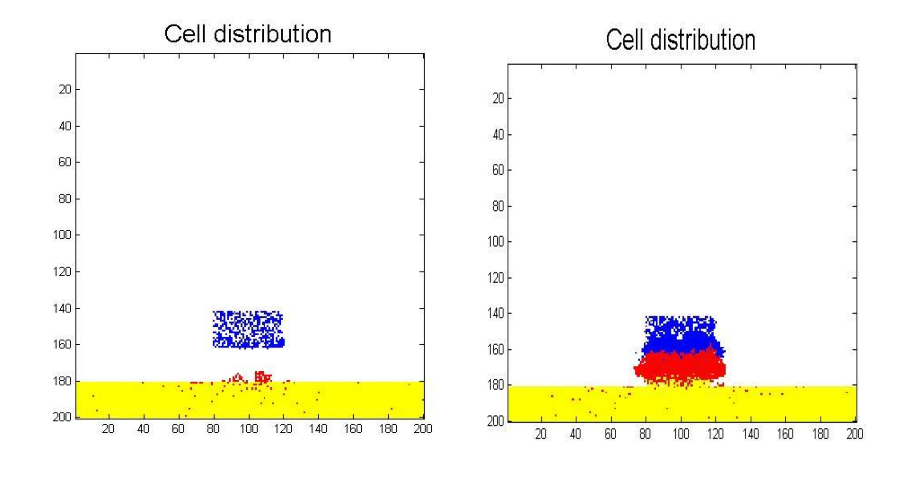
\includegraphics{bifucations.eps}}
\caption{}\label{fig:bifurcations}
\end{figure*} 


However, it is unlikely that this mechanism is the principal cause of branching \textit{in vivo}, since the mesenchyme are relatively diffuse. Thus they are unlikely to exert a sufficiently strong enough pressure on the wave of encroaching epithelium to halt the centre of the wavefront; allowing the growth laterally. Furthermore, \textit{in vitro} studies with explanted epithelium cells without mesenchyme have demonstrated that branching can continue to produce self-similar tips if GDNF is present \cite{qiao1999branching}. These two reasons cast serious doubt on this as a likely primary cause of branching. However, it may be the case that the pressure provided by the surrounding mesenchyme cap moderates the morphology of the developing UB, since the \textit{in vivo} and \textit{in vitro} branches are not the same.

\subsection{in vitro}
Symmetry is already broken \textit{in silico} for the initial transplanted epithelium mass. This meant that it was possible to initiate branch formation due to local minima in GDNF forming in clefts, and maxima at the outermost edges of the epithelium layer. The tips of the epithelium grew fastest due to GDNF-stimulated proliferation. By contrast those cells in pockets failed to grow since the surrounding epithelium cells had consumed a relatively high proportion of the GDNF. These tips hence became tentacles, extending outwards from the initial mass of epithelium cells.

Whilst branching was generated in the \textit{in vitro} simulations, it did not replicate the continued rounds of branching (across ranges or parameter values); each of which produces self-similar tips, which are witnessed in experiments. As such, the mechanism proposed here of an asymmetric mass of epithelium generating local maxima and minima in GDNF was not sufficient to replicate reality. Much like the \textit{in vivo} case, it will hence be necessary to investigate other causes of branching. In particular following Costantini and Koplan \cite{CostantiniFKopan2010}, it is believed that anisotrophic cell growth may hold the key to generating the  morphological patterns witnessed. This is further supported by work which suggests that there are differences between the proliferative habits of tip and trunk cells \cite{packard2013luminal}.

\section{Conclusion and future work}
The branching patterns that have been shown to result from simple GDNF-stimulated growth are not in exact accordance with reality. In particular the lack of continued rounds of branching in \textit{in silico} simulations for both the \textit{in vivo} and \textit{in vitro} models provide evidence that an important mechanism is being missed. Costantini and Koplan \cite{CostantiniFKopan2010} state that they believe that there are three potential mechanisms for generating the branching patterns seen in experiments: cell movements within the epithelium, orientated cell division, and changes of cell shape. It is the belief of the author that all three of these mechanisms likely play a role in branching, although anisotrophic growth between the tip and cap cells may be the most important. In the model formulation presented here, the lumen of the eventual collecting duct are not taken into account. This simplification may turn out to be important, since it may provide an axis around which epithelium cells can be applied a range of pressures. It is possible that the differential pressures exerted on the tip and trunk cells by the lumen may explain the difference in phenotype witnessed in their proliferation habits, and could be a potential cause of anisotrophic growth. Without including an explicit lumen, it is difficult to foresee how it would be possible to orientate cell division differently between the tip and trunk. Whilst it may be possible to explicitly include a lumen in a cellular automaton model, this may not be the most appropriate modelling framework to do so, and other cell-based models may be better.


\bibliographystyle{plain}
\bibliography{Kidney}


\end{document}